\documentclass[1p]{elsarticle_modified}
%\bibliographystyle{elsarticle-num}

%\usepackage[colorlinks]{hyperref}
%\usepackage{abbrmath_seonhwa} %\Abb, \Ascr, \Acal ,\Abf, \Afrak
\usepackage{amsfonts}
\usepackage{amssymb}
\usepackage{amsmath}
\usepackage{amsthm}
\usepackage{scalefnt}
\usepackage{amsbsy}
\usepackage{kotex}
\usepackage{caption}
\usepackage{subfig}
\usepackage{color}
\usepackage{graphicx}
\usepackage{xcolor} %% white, black, red, green, blue, cyan, magenta, yellow
\usepackage{float}
\usepackage{setspace}
\usepackage{hyperref}

\usepackage{tikz}
\usetikzlibrary{arrows}

\usepackage{multirow}
\usepackage{array} % fixed length table
\usepackage{hhline}

%%%%%%%%%%%%%%%%%%%%%
\makeatletter
\renewcommand*\env@matrix[1][\arraystretch]{%
	\edef\arraystretch{#1}%
	\hskip -\arraycolsep
	\let\@ifnextchar\new@ifnextchar
	\array{*\c@MaxMatrixCols c}}
\makeatother %https://tex.stackexchange.com/questions/14071/how-can-i-increase-the-line-spacing-in-a-matrix
%%%%%%%%%%%%%%%

\usepackage[normalem]{ulem}

\newcommand{\msout}[1]{\ifmmode\text{\sout{\ensuremath{#1}}}\else\sout{#1}\fi}
%SOURCE: \msout is \stkout macro in https://tex.stackexchange.com/questions/20609/strikeout-in-math-mode

\newcommand{\cancel}[1]{
	\ifmmode
	{\color{red}\msout{#1}}
	\else
	{\color{red}\sout{#1}}
	\fi
}

\newcommand{\add}[1]{
	{\color{blue}\uwave{#1}}
}

\newcommand{\replace}[2]{
	\ifmmode
	{\color{red}\msout{#1}}{\color{blue}\uwave{#2}}
	\else
	{\color{red}\sout{#1}}{\color{blue}\uwave{#2}}
	\fi
}

\newcommand{\Sol}{\mathcal{S}} %segment
\newcommand{\D}{D} %diagram
\newcommand{\A}{\mathcal{A}} %arc


%%%%%%%%%%%%%%%%%%%%%%%%%%%%%5 test

\def\sl{\operatorname{\textup{SL}}(2,\Cbb)}
\def\psl{\operatorname{\textup{PSL}}(2,\Cbb)}
\def\quan{\mkern 1mu \triangleright \mkern 1mu}

\theoremstyle{definition}
\newtheorem{thm}{Theorem}[section]
\newtheorem{prop}[thm]{Proposition}
\newtheorem{lem}[thm]{Lemma}
\newtheorem{ques}[thm]{Question}
\newtheorem{cor}[thm]{Corollary}
\newtheorem{defn}[thm]{Definition}
\newtheorem{exam}[thm]{Example}
\newtheorem{rmk}[thm]{Remark}
\newtheorem{alg}[thm]{Algorithm}

\newcommand{\I}{\sqrt{-1}}
\begin{document}

%\begin{frontmatter}
%
%\title{Boundary parabolic representations of knots up to 8 crossings}
%
%%% Group authors per affiliation:
%\author{Yunhi Cho} 
%\address{Department of Mathematics, University of Seoul, Seoul, Korea}
%\ead{yhcho@uos.ac.kr}
%
%
%\author{Seonhwa Kim} %\fnref{s_kim}}
%\address{Center for Geometry and Physics, Institute for Basic Science, Pohang, 37673, Korea}
%\ead{ryeona17@ibs.re.kr}
%
%\author{Hyuk Kim}
%\address{Department of Mathematical Sciences, Seoul National University, Seoul 08826, Korea}
%\ead{hyukkim@snu.ac.kr}
%
%\author{Seokbeom Yoon}
%\address{Department of Mathematical Sciences, Seoul National University, Seoul, 08826,  Korea}
%\ead{sbyoon15@snu.ac.kr}
%
%\begin{abstract}
%We find all boundary parabolic representation of knots up to 8 crossings.
%
%\end{abstract}
%\begin{keyword}
%    \MSC[2010] 57M25 
%\end{keyword}
%
%\end{frontmatter}

%\linenumbers
%\tableofcontents
%
\newcommand\colored[1]{\textcolor{white}{\rule[-0.35ex]{0.8em}{1.4ex}}\kern-0.8em\color{red} #1}%
%\newcommand\colored[1]{\textcolor{white}{ #1}\kern-2.17ex	\textcolor{white}{ #1}\kern-1.81ex	\textcolor{white}{ #1}\kern-2.15ex\color{red}#1	}

{\Large $\underline{12n_{0569}~(K12n_{0569})}$}

\setlength{\tabcolsep}{10pt}
\renewcommand{\arraystretch}{1.6}
\vspace{1cm}\begin{tabular}{m{100pt}>{\centering\arraybackslash}m{274pt}}
\multirow{5}{120pt}{
	\centering
	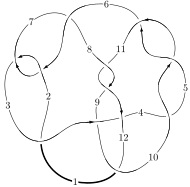
\includegraphics[width=112pt]{../../../GIT/diagram.site/Diagrams/png/2658_12n_0569.png}\\
\ \ \ A knot diagram\footnotemark}&
\allowdisplaybreaks
\textbf{Linearized knot diagam} \\
\cline{2-2}
 &
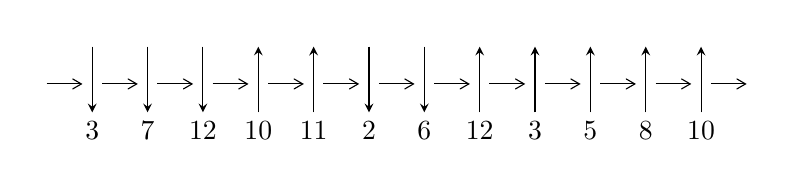
\begin{tikzpicture}[x=20pt, y=17pt]
	% nodes
	\node (C0) at (0, 0) {};
	\node (C1) at (1, 0) {};
	\node (C1U) at (1, +1) {};
	\node (C1D) at (1, -1) {3};

	\node (C2) at (2, 0) {};
	\node (C2U) at (2, +1) {};
	\node (C2D) at (2, -1) {7};

	\node (C3) at (3, 0) {};
	\node (C3U) at (3, +1) {};
	\node (C3D) at (3, -1) {12};

	\node (C4) at (4, 0) {};
	\node (C4U) at (4, +1) {};
	\node (C4D) at (4, -1) {10};

	\node (C5) at (5, 0) {};
	\node (C5U) at (5, +1) {};
	\node (C5D) at (5, -1) {11};

	\node (C6) at (6, 0) {};
	\node (C6U) at (6, +1) {};
	\node (C6D) at (6, -1) {2};

	\node (C7) at (7, 0) {};
	\node (C7U) at (7, +1) {};
	\node (C7D) at (7, -1) {6};

	\node (C8) at (8, 0) {};
	\node (C8U) at (8, +1) {};
	\node (C8D) at (8, -1) {12};

	\node (C9) at (9, 0) {};
	\node (C9U) at (9, +1) {};
	\node (C9D) at (9, -1) {3};

	\node (C10) at (10, 0) {};
	\node (C10U) at (10, +1) {};
	\node (C10D) at (10, -1) {5};

	\node (C11) at (11, 0) {};
	\node (C11U) at (11, +1) {};
	\node (C11D) at (11, -1) {8};

	\node (C12) at (12, 0) {};
	\node (C12U) at (12, +1) {};
	\node (C12D) at (12, -1) {10};
	\node (C13) at (13, 0) {};

	% arrows
	\draw[->,>={angle 60}]
	(C0) edge (C1) (C1) edge (C2) (C2) edge (C3) (C3) edge (C4) (C4) edge (C5) (C5) edge (C6) (C6) edge (C7) (C7) edge (C8) (C8) edge (C9) (C9) edge (C10) (C10) edge (C11) (C11) edge (C12) (C12) edge (C13) ;	\draw[->,>=stealth]
	(C1U) edge (C1D) (C2U) edge (C2D) (C3U) edge (C3D) (C4D) edge (C4U) (C5D) edge (C5U) (C6U) edge (C6D) (C7U) edge (C7D) (C8D) edge (C8U) (C9D) edge (C9U) (C10D) edge (C10U) (C11D) edge (C11U) (C12D) edge (C12U) ;
	\end{tikzpicture} \\
\hhline{~~} \\& 
\textbf{Solving Sequence} \\ \cline{2-2} 
 &
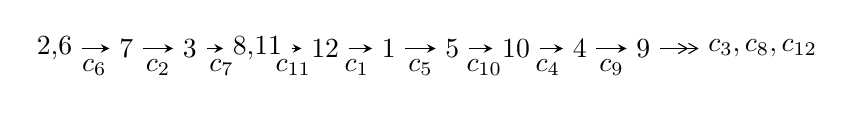
\begin{tikzpicture}[x=23pt, y=7pt]
	% node
	\node (A0) at (-1/8, 0) {2,6};
	\node (A1) at (1, 0) {7};
	\node (A2) at (2, 0) {3};
	\node (A3) at (49/16, 0) {8,11};
	\node (A4) at (33/8, 0) {12};
	\node (A5) at (41/8, 0) {1};
	\node (A6) at (49/8, 0) {5};
	\node (A7) at (57/8, 0) {10};
	\node (A8) at (65/8, 0) {4};
	\node (A9) at (73/8, 0) {9};
	\node (C1) at (1/2, -1) {$c_{6}$};
	\node (C2) at (3/2, -1) {$c_{2}$};
	\node (C3) at (5/2, -1) {$c_{7}$};
	\node (C4) at (29/8, -1) {$c_{11}$};
	\node (C5) at (37/8, -1) {$c_{1}$};
	\node (C6) at (45/8, -1) {$c_{5}$};
	\node (C7) at (53/8, -1) {$c_{10}$};
	\node (C8) at (61/8, -1) {$c_{4}$};
	\node (C9) at (69/8, -1) {$c_{9}$};
	\node (A10) at (11, 0) {$c_{3},c_{8},c_{12}$};

	% edge
	\draw[->,>=stealth]	
	(A0) edge (A1) (A1) edge (A2) (A2) edge (A3) (A3) edge (A4) (A4) edge (A5) (A5) edge (A6) (A6) edge (A7) (A7) edge (A8) (A8) edge (A9) ;
	\draw[->>,>={angle 60}]	
	(A9) edge (A10);
\end{tikzpicture} \\ 

\end{tabular} \\

\footnotetext{
The image of knot diagram is generated by the software ``\textbf{Draw programme}" developed by Andrew Bartholomew(\url{http://www.layer8.co.uk/maths/draw/index.htm\#Running-draw}), where we modified some parts for our purpose(\url{https://github.com/CATsTAILs/LinksPainter}).
}\phantom \\ \newline 
\centering \textbf{Ideals for irreducible components\footnotemark of $X_{\text{par}}$} 
 
\begin{align*}
I^u_{1}&=\langle 
8.11108\times10^{37} u^{57}+4.91027\times10^{37} u^{56}+\cdots+5.66410\times10^{38} b-1.34973\times10^{39},\\
\phantom{I^u_{1}}&\phantom{= \langle  }1.29757\times10^{39} u^{57}+3.25753\times10^{39} u^{56}+\cdots+5.66410\times10^{38} a-5.91852\times10^{37},\;u^{58}+2 u^{57}+\cdots-9 u-1\rangle \\
I^u_{2}&=\langle 
u^{15}+u^{14}-3 u^{13}-4 u^{12}+7 u^{11}+10 u^{10}-10 u^9-16 u^8+11 u^7+19 u^6-8 u^5-15 u^4+4 u^3+7 u^2+b-2 u-2,\\
\phantom{I^u_{2}}&\phantom{= \langle  }-2 u^{16}- u^{15}+\cdots+a+1,\;u^{17}+u^{16}+\cdots-5 u^2+1\rangle \\
\\
\end{align*}
\raggedright * 2 irreducible components of $\dim_{\mathbb{C}}=0$, with total 75 representations.\\
\footnotetext{All coefficients of polynomials are rational numbers. But the coefficients are sometimes approximated in decimal forms when there is not enough margin.}
\newpage
\renewcommand{\arraystretch}{1}
\centering \section*{I. $I^u_{1}= \langle 8.11\times10^{37} u^{57}+4.91\times10^{37} u^{56}+\cdots+5.66\times10^{38} b-1.35\times10^{39},\;1.30\times10^{39} u^{57}+3.26\times10^{39} u^{56}+\cdots+5.66\times10^{38} a-5.92\times10^{37},\;u^{58}+2 u^{57}+\cdots-9 u-1 \rangle$}
\flushleft \textbf{(i) Arc colorings}\\
\begin{tabular}{m{7pt} m{180pt} m{7pt} m{180pt} }
\flushright $a_{2}=$&$\begin{pmatrix}0\\u\end{pmatrix}$ \\
\flushright $a_{6}=$&$\begin{pmatrix}1\\0\end{pmatrix}$ \\
\flushright $a_{7}=$&$\begin{pmatrix}1\\u^2\end{pmatrix}$ \\
\flushright $a_{3}=$&$\begin{pmatrix}- u\\- u^3+u\end{pmatrix}$ \\
\flushright $a_{8}=$&$\begin{pmatrix}- u^2+1\\u^2\end{pmatrix}$ \\
\flushright $a_{11}=$&$\begin{pmatrix}-2.29087 u^{57}-5.75119 u^{56}+\cdots-44.7958 u+0.104492\\-0.143202 u^{57}-0.0866910 u^{56}+\cdots+6.22932 u+2.38295\end{pmatrix}$ \\
\flushright $a_{12}=$&$\begin{pmatrix}-1.52712 u^{57}-4.39667 u^{56}+\cdots-31.5613 u+3.08463\\-0.103380 u^{57}+0.538492 u^{56}+\cdots+10.3860 u+2.75551\end{pmatrix}$ \\
\flushright $a_{1}=$&$\begin{pmatrix}u^3\\u^5- u^3+u\end{pmatrix}$ \\
\flushright $a_{5}=$&$\begin{pmatrix}-1.60930 u^{57}-3.86858 u^{56}+\cdots-1.74961 u+7.98100\\1.09318 u^{57}+2.32144 u^{56}+\cdots+8.84503 u+3.47131\end{pmatrix}$ \\
\flushright $a_{10}=$&$\begin{pmatrix}-1.14552 u^{57}-4.13737 u^{56}+\cdots-72.7081 u-15.0427\\-0.129885 u^{57}+0.333506 u^{56}+\cdots-3.41712 u-2.96099\end{pmatrix}$ \\
\flushright $a_{4}=$&$\begin{pmatrix}-2.16693 u^{57}-5.96581 u^{56}+\cdots-57.6969 u-9.85977\\0.892300 u^{57}+1.86393 u^{56}+\cdots+9.09728 u-0.642831\end{pmatrix}$ \\
\flushright $a_{9}=$&$\begin{pmatrix}-0.697310 u^{57}-3.28572 u^{56}+\cdots-62.1886 u-13.9750\\-0.544392 u^{57}-0.342782 u^{56}+\cdots-13.8913 u-4.07349\end{pmatrix}$\\&\end{tabular}
\flushleft \textbf{(ii) Obstruction class $= -1$}\\~\\
\flushleft \textbf{(iii) Cusp Shapes $= -4.70530 u^{57}-10.9734 u^{56}+\cdots-119.055 u+7.76720$}\\~\\
\newpage\renewcommand{\arraystretch}{1}
\flushleft \textbf{(iv) u-Polynomials at the component}\newline \\
\begin{tabular}{m{50pt}|m{274pt}}
Crossings & \hspace{64pt}u-Polynomials at each crossing \\
\hline $$\begin{aligned}c_{1},c_{7}\end{aligned}$$&$\begin{aligned}
&u^{58}+20 u^{57}+\cdots+111 u+1
\end{aligned}$\\
\hline $$\begin{aligned}c_{2},c_{6}\end{aligned}$$&$\begin{aligned}
&u^{58}-2 u^{57}+\cdots+9 u-1
\end{aligned}$\\
\hline $$\begin{aligned}c_{3}\end{aligned}$$&$\begin{aligned}
&u^{58}-2 u^{57}+\cdots-4 u+1
\end{aligned}$\\
\hline $$\begin{aligned}c_{4},c_{5},c_{10}\end{aligned}$$&$\begin{aligned}
&u^{58}+u^{57}+\cdots-148 u-43
\end{aligned}$\\
\hline $$\begin{aligned}c_{8},c_{11}\end{aligned}$$&$\begin{aligned}
&u^{58}-4 u^{57}+\cdots+12848 u-2119
\end{aligned}$\\
\hline $$\begin{aligned}c_{9}\end{aligned}$$&$\begin{aligned}
&u^{58}- u^{57}+\cdots+2150 u+293
\end{aligned}$\\
\hline $$\begin{aligned}c_{12}\end{aligned}$$&$\begin{aligned}
&u^{58}+2 u^{57}+\cdots+44 u+1
\end{aligned}$\\
\hline
\end{tabular}\\~\\
\newpage\renewcommand{\arraystretch}{1}
\flushleft \textbf{(v) Riley Polynomials at the component}\newline \\
\begin{tabular}{m{50pt}|m{274pt}}
Crossings & \hspace{64pt}Riley Polynomials at each crossing \\
\hline $$\begin{aligned}c_{1},c_{7}\end{aligned}$$&$\begin{aligned}
&y^{58}+44 y^{57}+\cdots-6891 y+1
\end{aligned}$\\
\hline $$\begin{aligned}c_{2},c_{6}\end{aligned}$$&$\begin{aligned}
&y^{58}-20 y^{57}+\cdots-111 y+1
\end{aligned}$\\
\hline $$\begin{aligned}c_{3}\end{aligned}$$&$\begin{aligned}
&y^{58}-56 y^{57}+\cdots+254 y+1
\end{aligned}$\\
\hline $$\begin{aligned}c_{4},c_{5},c_{10}\end{aligned}$$&$\begin{aligned}
&y^{58}-57 y^{57}+\cdots+10690 y+1849
\end{aligned}$\\
\hline $$\begin{aligned}c_{8},c_{11}\end{aligned}$$&$\begin{aligned}
&y^{58}-34 y^{57}+\cdots-42707330 y+4490161
\end{aligned}$\\
\hline $$\begin{aligned}c_{9}\end{aligned}$$&$\begin{aligned}
&y^{58}+55 y^{57}+\cdots-1142832 y+85849
\end{aligned}$\\
\hline $$\begin{aligned}c_{12}\end{aligned}$$&$\begin{aligned}
&y^{58}+50 y^{57}+\cdots+2238 y+1
\end{aligned}$\\
\hline
\end{tabular}\\~\\
\newpage\flushleft \textbf{(vi) Complex Volumes and Cusp Shapes}
$$\begin{array}{c|c|c}  
\text{Solutions to }I^u_{1}& \I (\text{vol} + \sqrt{-1}CS) & \text{Cusp shape}\\
 \hline 
\begin{aligned}
u &= -0.649208 + 0.777185 I \\
a &= -1.311830 - 0.015356 I \\
b &= \phantom{-}1.41367 - 0.24080 I\end{aligned}
 & \phantom{-}8.99829 - 0.85807 I & \phantom{-}7.14206 + 0. I\phantom{ +0.000000I} \\ \hline\begin{aligned}
u &= -0.649208 - 0.777185 I \\
a &= -1.311830 + 0.015356 I \\
b &= \phantom{-}1.41367 + 0.24080 I\end{aligned}
 & \phantom{-}8.99829 + 0.85807 I & \phantom{-}7.14206 + 0. I\phantom{ +0.000000I} \\ \hline\begin{aligned}
u &= -0.192605 + 0.952386 I \\
a &= \phantom{-}1.59370 + 0.08023 I \\
b &= -1.374660 - 0.179161 I\end{aligned}
 & \phantom{-}1.95932 + 3.47319 I & \phantom{-}7.38337 - 3.16681 I \\ \hline\begin{aligned}
u &= -0.192605 - 0.952386 I \\
a &= \phantom{-}1.59370 - 0.08023 I \\
b &= -1.374660 + 0.179161 I\end{aligned}
 & \phantom{-}1.95932 - 3.47319 I & \phantom{-}7.38337 + 3.16681 I \\ \hline\begin{aligned}
u &= \phantom{-}0.704542 + 0.759694 I \\
a &= -2.20492 - 0.44914 I \\
b &= \phantom{-}1.66369 + 0.08603 I\end{aligned}
 & \phantom{-}9.70913 + 0.22811 I & \phantom{-}5.29825 + 0. I\phantom{ +0.000000I} \\ \hline\begin{aligned}
u &= \phantom{-}0.704542 - 0.759694 I \\
a &= -2.20492 + 0.44914 I \\
b &= \phantom{-}1.66369 - 0.08603 I\end{aligned}
 & \phantom{-}9.70913 - 0.22811 I & \phantom{-}5.29825 + 0. I\phantom{ +0.000000I} \\ \hline\begin{aligned}
u &= -0.844133 + 0.459005 I \\
a &= -0.88197 + 1.28310 I \\
b &= \phantom{-}0.794410 + 0.348082 I\end{aligned}
 & \phantom{-}0.18156 + 3.43068 I & \phantom{-}3.97292 - 8.38855 I \\ \hline\begin{aligned}
u &= -0.844133 - 0.459005 I \\
a &= -0.88197 - 1.28310 I \\
b &= \phantom{-}0.794410 - 0.348082 I\end{aligned}
 & \phantom{-}0.18156 - 3.43068 I & \phantom{-}3.97292 + 8.38855 I \\ \hline\begin{aligned}
u &= -0.785206 + 0.690856 I \\
a &= -1.51273 + 0.86981 I \\
b &= \phantom{-}0.940956 + 0.796608 I\end{aligned}
 & \phantom{-}0.04805 + 2.72947 I & \phantom{-}6.00584 - 3.68019 I \\ \hline\begin{aligned}
u &= -0.785206 - 0.690856 I \\
a &= -1.51273 - 0.86981 I \\
b &= \phantom{-}0.940956 - 0.796608 I\end{aligned}
 & \phantom{-}0.04805 - 2.72947 I & \phantom{-}6.00584 + 3.68019 I\\
 \hline 
 \end{array}$$\newpage$$\begin{array}{c|c|c}  
\text{Solutions to }I^u_{1}& \I (\text{vol} + \sqrt{-1}CS) & \text{Cusp shape}\\
 \hline 
\begin{aligned}
u &= \phantom{-}0.675145 + 0.804414 I \\
a &= \phantom{-}0.143408 - 0.529642 I \\
b &= \phantom{-}0.449289 + 0.991573 I\end{aligned}
 & -1.36150 + 3.46891 I & \phantom{-}4.09542 - 2.58287 I \\ \hline\begin{aligned}
u &= \phantom{-}0.675145 - 0.804414 I \\
a &= \phantom{-}0.143408 + 0.529642 I \\
b &= \phantom{-}0.449289 - 0.991573 I\end{aligned}
 & -1.36150 - 3.46891 I & \phantom{-}4.09542 + 2.58287 I \\ \hline\begin{aligned}
u &= -1.06579\phantom{ +0.000000I} \\
a &= -0.471638\phantom{ +0.000000I} \\
b &= -1.49871\phantom{ +0.000000I}\end{aligned}
 & \phantom{-}4.21383\phantom{ +0.000000I} & -2.91260\phantom{ +0.000000I} \\ \hline\begin{aligned}
u &= -0.797269 + 0.746574 I \\
a &= -2.49041 + 1.51484 I \\
b &= \phantom{-}1.313240 - 0.095807 I\end{aligned}
 & \phantom{-}0.640941 - 0.368761 I & \phantom{-0.000000 } 0 \\ \hline\begin{aligned}
u &= -0.797269 - 0.746574 I \\
a &= -2.49041 - 1.51484 I \\
b &= \phantom{-}1.313240 + 0.095807 I\end{aligned}
 & \phantom{-}0.640941 + 0.368761 I & \phantom{-0.000000 } 0 \\ \hline\begin{aligned}
u &= -1.093130 + 0.112916 I \\
a &= -0.372147 - 0.718737 I \\
b &= -0.097432 - 0.849324 I\end{aligned}
 & -7.71465 + 3.17136 I & \phantom{-0.000000 } 0. - 3.24101 I \\ \hline\begin{aligned}
u &= -1.093130 - 0.112916 I \\
a &= -0.372147 + 0.718737 I \\
b &= -0.097432 + 0.849324 I\end{aligned}
 & -7.71465 - 3.17136 I & \phantom{-0.000000 -}0. + 3.24101 I \\ \hline\begin{aligned}
u &= \phantom{-}0.897438 + 0.025837 I \\
a &= \phantom{-}0.83649 + 1.36225 I \\
b &= -1.246550 + 0.521890 I\end{aligned}
 & -4.22900 - 1.73682 I & -1.19489 + 1.04559 I \\ \hline\begin{aligned}
u &= \phantom{-}0.897438 - 0.025837 I \\
a &= \phantom{-}0.83649 - 1.36225 I \\
b &= -1.246550 - 0.521890 I\end{aligned}
 & -4.22900 + 1.73682 I & -1.19489 - 1.04559 I \\ \hline\begin{aligned}
u &= \phantom{-}0.865118 + 0.692108 I \\
a &= -0.329927 - 0.483809 I \\
b &= -0.099466 - 0.733477 I\end{aligned}
 & \phantom{-}3.97645 - 2.66265 I & \phantom{-0.000000 } 0\\
 \hline 
 \end{array}$$\newpage$$\begin{array}{c|c|c}  
\text{Solutions to }I^u_{1}& \I (\text{vol} + \sqrt{-1}CS) & \text{Cusp shape}\\
 \hline 
\begin{aligned}
u &= \phantom{-}0.865118 - 0.692108 I \\
a &= -0.329927 + 0.483809 I \\
b &= -0.099466 + 0.733477 I\end{aligned}
 & \phantom{-}3.97645 + 2.66265 I & \phantom{-0.000000 } 0 \\ \hline\begin{aligned}
u &= \phantom{-}1.12004\phantom{ +0.000000I} \\
a &= -0.852945\phantom{ +0.000000I} \\
b &= -1.22513\phantom{ +0.000000I}\end{aligned}
 & \phantom{-}3.22886\phantom{ +0.000000I} & \phantom{-}2.00000\phantom{ +0.000000I} \\ \hline\begin{aligned}
u &= -0.927826 + 0.684508 I \\
a &= \phantom{-}0.367169 - 0.609308 I \\
b &= -1.072260 + 0.836652 I\end{aligned}
 & -0.38663 + 2.57641 I & \phantom{-0.000000 } 0 \\ \hline\begin{aligned}
u &= -0.927826 - 0.684508 I \\
a &= \phantom{-}0.367169 + 0.609308 I \\
b &= -1.072260 - 0.836652 I\end{aligned}
 & -0.38663 - 2.57641 I & \phantom{-0.000000 } 0 \\ \hline\begin{aligned}
u &= -0.671464 + 0.950623 I \\
a &= \phantom{-}1.75527 - 0.30187 I \\
b &= -1.53135 + 0.36764 I\end{aligned}
 & \phantom{-}5.01980 - 8.36674 I & \phantom{-0.000000 } 0 \\ \hline\begin{aligned}
u &= -0.671464 - 0.950623 I \\
a &= \phantom{-}1.75527 + 0.30187 I \\
b &= -1.53135 - 0.36764 I\end{aligned}
 & \phantom{-}5.01980 + 8.36674 I & \phantom{-0.000000 } 0 \\ \hline\begin{aligned}
u &= \phantom{-}0.813233 + 0.191671 I \\
a &= \phantom{-}0.451115 + 0.585998 I \\
b &= \phantom{-}0.221008 + 0.395351 I\end{aligned}
 & -1.37591 - 0.60280 I & -3.98558 + 1.14738 I \\ \hline\begin{aligned}
u &= \phantom{-}0.813233 - 0.191671 I \\
a &= \phantom{-}0.451115 - 0.585998 I \\
b &= \phantom{-}0.221008 - 0.395351 I\end{aligned}
 & -1.37591 + 0.60280 I & -3.98558 - 1.14738 I \\ \hline\begin{aligned}
u &= -0.938275 + 0.718133 I \\
a &= \phantom{-}2.51455 - 0.78526 I \\
b &= -1.40735 - 0.18115 I\end{aligned}
 & \phantom{-}0.20384 + 5.94515 I & \phantom{-0.000000 } 0 \\ \hline\begin{aligned}
u &= -0.938275 - 0.718133 I \\
a &= \phantom{-}2.51455 + 0.78526 I \\
b &= -1.40735 + 0.18115 I\end{aligned}
 & \phantom{-}0.20384 - 5.94515 I & \phantom{-0.000000 } 0\\
 \hline 
 \end{array}$$\newpage$$\begin{array}{c|c|c}  
\text{Solutions to }I^u_{1}& \I (\text{vol} + \sqrt{-1}CS) & \text{Cusp shape}\\
 \hline 
\begin{aligned}
u &= \phantom{-}0.400647 + 0.687623 I \\
a &= \phantom{-}0.654871 + 0.604463 I \\
b &= \phantom{-}0.179950 - 0.417028 I\end{aligned}
 & -3.03619 - 1.14742 I & \phantom{-}1.89413 + 2.71155 I \\ \hline\begin{aligned}
u &= \phantom{-}0.400647 - 0.687623 I \\
a &= \phantom{-}0.654871 - 0.604463 I \\
b &= \phantom{-}0.179950 + 0.417028 I\end{aligned}
 & -3.03619 + 1.14742 I & \phantom{-}1.89413 - 2.71155 I \\ \hline\begin{aligned}
u &= \phantom{-}1.068030 + 0.569719 I \\
a &= -1.042390 + 0.124560 I \\
b &= \phantom{-}0.140212 - 0.417001 I\end{aligned}
 & -4.94353 - 3.70127 I & \phantom{-0.000000 } 0 \\ \hline\begin{aligned}
u &= \phantom{-}1.068030 - 0.569719 I \\
a &= -1.042390 - 0.124560 I \\
b &= \phantom{-}0.140212 + 0.417001 I\end{aligned}
 & -4.94353 + 3.70127 I & \phantom{-0.000000 } 0 \\ \hline\begin{aligned}
u &= -0.899742 + 0.819342 I \\
a &= \phantom{-}0.385454 - 0.035512 I \\
b &= \phantom{-}0.037648 - 0.622247 I\end{aligned}
 & \phantom{-}4.54646 + 3.06184 I & \phantom{-0.000000 } 0 \\ \hline\begin{aligned}
u &= -0.899742 - 0.819342 I \\
a &= \phantom{-}0.385454 + 0.035512 I \\
b &= \phantom{-}0.037648 + 0.622247 I\end{aligned}
 & \phantom{-}4.54646 - 3.06184 I & \phantom{-0.000000 } 0 \\ \hline\begin{aligned}
u &= \phantom{-}0.998592 + 0.706419 I \\
a &= \phantom{-}1.64774 + 1.70115 I \\
b &= -1.63453 + 0.16359 I\end{aligned}
 & \phantom{-}8.81746 - 5.81212 I & \phantom{-0.000000 } 0 \\ \hline\begin{aligned}
u &= \phantom{-}0.998592 - 0.706419 I \\
a &= \phantom{-}1.64774 - 1.70115 I \\
b &= -1.63453 - 0.16359 I\end{aligned}
 & \phantom{-}8.81746 + 5.81212 I & \phantom{-0.000000 } 0 \\ \hline\begin{aligned}
u &= -1.029770 + 0.700716 I \\
a &= \phantom{-}1.01570 - 1.60259 I \\
b &= -1.311010 - 0.312734 I\end{aligned}
 & \phantom{-}7.85730 + 6.47303 I & \phantom{-0.000000 } 0 \\ \hline\begin{aligned}
u &= -1.029770 - 0.700716 I \\
a &= \phantom{-}1.01570 + 1.60259 I \\
b &= -1.311010 + 0.312734 I\end{aligned}
 & \phantom{-}7.85730 - 6.47303 I & \phantom{-0.000000 } 0\\
 \hline 
 \end{array}$$\newpage$$\begin{array}{c|c|c}  
\text{Solutions to }I^u_{1}& \I (\text{vol} + \sqrt{-1}CS) & \text{Cusp shape}\\
 \hline 
\begin{aligned}
u &= \phantom{-}1.018850 + 0.717395 I \\
a &= \phantom{-}1.035050 + 0.243093 I \\
b &= -0.380419 + 1.097530 I\end{aligned}
 & -2.39802 - 9.20313 I & \phantom{-0.000000 } 0 \\ \hline\begin{aligned}
u &= \phantom{-}1.018850 - 0.717395 I \\
a &= \phantom{-}1.035050 - 0.243093 I \\
b &= -0.380419 - 1.097530 I\end{aligned}
 & -2.39802 + 9.20313 I & \phantom{-0.000000 } 0 \\ \hline\begin{aligned}
u &= \phantom{-}0.853820 + 0.915715 I \\
a &= \phantom{-}1.68680 + 0.32381 I \\
b &= -1.367730 - 0.197646 I\end{aligned}
 & \phantom{-}9.17939 - 0.17615 I & \phantom{-0.000000 } 0 \\ \hline\begin{aligned}
u &= \phantom{-}0.853820 - 0.915715 I \\
a &= \phantom{-}1.68680 - 0.32381 I \\
b &= -1.367730 + 0.197646 I\end{aligned}
 & \phantom{-}9.17939 + 0.17615 I & \phantom{-0.000000 } 0 \\ \hline\begin{aligned}
u &= \phantom{-}1.245010 + 0.220439 I \\
a &= -0.109370 - 0.713094 I \\
b &= \phantom{-}1.355710 - 0.323925 I\end{aligned}
 & -3.11278 - 7.32391 I & \phantom{-0.000000 } 0 \\ \hline\begin{aligned}
u &= \phantom{-}1.245010 - 0.220439 I \\
a &= -0.109370 + 0.713094 I \\
b &= \phantom{-}1.355710 + 0.323925 I\end{aligned}
 & -3.11278 + 7.32391 I & \phantom{-0.000000 } 0 \\ \hline\begin{aligned}
u &= \phantom{-}0.979010 + 0.852448 I \\
a &= -1.77380 - 1.22586 I \\
b &= \phantom{-}1.340370 - 0.264461 I\end{aligned}
 & \phantom{-}8.77545 - 6.33818 I & \phantom{-0.000000 } 0 \\ \hline\begin{aligned}
u &= \phantom{-}0.979010 - 0.852448 I \\
a &= -1.77380 + 1.22586 I \\
b &= \phantom{-}1.340370 + 0.264461 I\end{aligned}
 & \phantom{-}8.77545 + 6.33818 I & \phantom{-0.000000 } 0 \\ \hline\begin{aligned}
u &= -1.212290 + 0.502784 I \\
a &= -0.308235 + 0.936072 I \\
b &= \phantom{-}1.265380 - 0.139334 I\end{aligned}
 & -1.33691 + 1.73049 I & \phantom{-0.000000 } 0 \\ \hline\begin{aligned}
u &= -1.212290 - 0.502784 I \\
a &= -0.308235 - 0.936072 I \\
b &= \phantom{-}1.265380 + 0.139334 I\end{aligned}
 & -1.33691 - 1.73049 I & \phantom{-0.000000 } 0\\
 \hline 
 \end{array}$$\newpage$$\begin{array}{c|c|c}  
\text{Solutions to }I^u_{1}& \I (\text{vol} + \sqrt{-1}CS) & \text{Cusp shape}\\
 \hline 
\begin{aligned}
u &= -0.606543 + 0.302471 I \\
a &= \phantom{-}1.286880 - 0.357784 I \\
b &= -0.620734 - 0.064910 I\end{aligned}
 & \phantom{-}0.958498 + 0.031162 I & \phantom{-}9.31326 - 1.44144 I \\ \hline\begin{aligned}
u &= -0.606543 - 0.302471 I \\
a &= \phantom{-}1.286880 + 0.357784 I \\
b &= -0.620734 + 0.064910 I\end{aligned}
 & \phantom{-}0.958498 - 0.031162 I & \phantom{-}9.31326 + 1.44144 I \\ \hline\begin{aligned}
u &= -1.079880 + 0.772455 I \\
a &= -1.65559 + 1.44153 I \\
b &= \phantom{-}1.53699 + 0.42805 I\end{aligned}
 & \phantom{-}3.7392 + 14.6910 I & \phantom{-0.000000 } 0 \\ \hline\begin{aligned}
u &= -1.079880 - 0.772455 I \\
a &= -1.65559 - 1.44153 I \\
b &= \phantom{-}1.53699 - 0.42805 I\end{aligned}
 & \phantom{-}3.7392 - 14.6910 I & \phantom{-0.000000 } 0 \\ \hline\begin{aligned}
u &= \phantom{-}0.453560 + 0.034976 I \\
a &= \phantom{-}3.14159 + 1.95342 I \\
b &= \phantom{-}0.810649 - 0.339207 I\end{aligned}
 & -2.55565 - 1.59256 I & -2.14433 + 3.75237 I \\ \hline\begin{aligned}
u &= \phantom{-}0.453560 - 0.034976 I \\
a &= \phantom{-}3.14159 - 1.95342 I \\
b &= \phantom{-}0.810649 + 0.339207 I\end{aligned}
 & -2.55565 + 1.59256 I & -2.14433 - 3.75237 I \\ \hline\begin{aligned}
u &= -0.435557\phantom{ +0.000000I} \\
a &= \phantom{-}1.52560\phantom{ +0.000000I} \\
b &= -0.476437\phantom{ +0.000000I}\end{aligned}
 & \phantom{-}0.883998\phantom{ +0.000000I} & \phantom{-}12.6720\phantom{ +0.000000I} \\ \hline\begin{aligned}
u &= -0.109994\phantom{ +0.000000I} \\
a &= \phantom{-}3.75403\phantom{ +0.000000I} \\
b &= \phantom{-}1.56091\phantom{ +0.000000I}\end{aligned}
 & \phantom{-}7.69349\phantom{ +0.000000I} & \phantom{-}17.3580\phantom{ +0.000000I}\\
 \hline 
 \end{array}$$\newpage\newpage\renewcommand{\arraystretch}{1}
\centering \section*{II. $I^u_{2}= \langle u^{15}+u^{14}+\cdots+b-2,\;-2 u^{16}- u^{15}+\cdots+a+1,\;u^{17}+u^{16}+\cdots-5 u^2+1 \rangle$}
\flushleft \textbf{(i) Arc colorings}\\
\begin{tabular}{m{7pt} m{180pt} m{7pt} m{180pt} }
\flushright $a_{2}=$&$\begin{pmatrix}0\\u\end{pmatrix}$ \\
\flushright $a_{6}=$&$\begin{pmatrix}1\\0\end{pmatrix}$ \\
\flushright $a_{7}=$&$\begin{pmatrix}1\\u^2\end{pmatrix}$ \\
\flushright $a_{3}=$&$\begin{pmatrix}- u\\- u^3+u\end{pmatrix}$ \\
\flushright $a_{8}=$&$\begin{pmatrix}- u^2+1\\u^2\end{pmatrix}$ \\
\flushright $a_{11}=$&$\begin{pmatrix}2 u^{16}+u^{15}+\cdots-2 u-1\\- u^{15}- u^{14}+\cdots+2 u+2\end{pmatrix}$ \\
\flushright $a_{12}=$&$\begin{pmatrix}u^{16}-3 u^{14}+\cdots+u-1\\- u^{15}- u^{14}+\cdots+3 u+2\end{pmatrix}$ \\
\flushright $a_{1}=$&$\begin{pmatrix}u^3\\u^5- u^3+u\end{pmatrix}$ \\
\flushright $a_{5}=$&$\begin{pmatrix}- u^{16}+4 u^{14}+\cdots-3 u-1\\- u^{16}- u^{15}+\cdots+4 u+1\end{pmatrix}$ \\
\flushright $a_{10}=$&$\begin{pmatrix}- u^{16}- u^{15}+\cdots+u-1\\u^{16}+u^{15}+\cdots-2 u-2\end{pmatrix}$ \\
\flushright $a_{4}=$&$\begin{pmatrix}- u^{16}+3 u^{14}+\cdots-3 u+2\\u^{15}+u^{14}+\cdots-2 u-2\end{pmatrix}$ \\
\flushright $a_{9}=$&$\begin{pmatrix}- u^{16}- u^{15}+\cdots+5 u^2+u\\u^{16}+u^{15}+\cdots-2 u-3\end{pmatrix}$\\&\end{tabular}
\flushleft \textbf{(ii) Obstruction class $= 1$}\\~\\
\flushleft \textbf{(iii) Cusp Shapes $= -2 u^{16}+4 u^{15}+8 u^{14}-9 u^{13}-25 u^{12}+22 u^{11}+46 u^{10}-26 u^9-69 u^8+31 u^7+73 u^6-19 u^5-62 u^4+15 u^3+32 u^2-5 u-10$}\\~\\
\newpage\renewcommand{\arraystretch}{1}
\flushleft \textbf{(iv) u-Polynomials at the component}\newline \\
\begin{tabular}{m{50pt}|m{274pt}}
Crossings & \hspace{64pt}u-Polynomials at each crossing \\
\hline $$\begin{aligned}c_{1}\end{aligned}$$&$\begin{aligned}
&u^{17}-7 u^{16}+\cdots+10 u-1
\end{aligned}$\\
\hline $$\begin{aligned}c_{2}\end{aligned}$$&$\begin{aligned}
&u^{17}- u^{16}+\cdots+5 u^2-1
\end{aligned}$\\
\hline $$\begin{aligned}c_{3}\end{aligned}$$&$\begin{aligned}
&u^{17}+3 u^{16}+\cdots+5 u-1
\end{aligned}$\\
\hline $$\begin{aligned}c_{4},c_{5}\end{aligned}$$&$\begin{aligned}
&u^{17}-10 u^{15}+\cdots-5 u-1
\end{aligned}$\\
\hline $$\begin{aligned}c_{6}\end{aligned}$$&$\begin{aligned}
&u^{17}+u^{16}+\cdots-5 u^2+1
\end{aligned}$\\
\hline $$\begin{aligned}c_{7}\end{aligned}$$&$\begin{aligned}
&u^{17}+7 u^{16}+\cdots+10 u+1
\end{aligned}$\\
\hline $$\begin{aligned}c_{8}\end{aligned}$$&$\begin{aligned}
&u^{17}-3 u^{16}+\cdots+u+1
\end{aligned}$\\
\hline $$\begin{aligned}c_{9}\end{aligned}$$&$\begin{aligned}
&u^{17}+4 u^{15}+\cdots-5 u-1
\end{aligned}$\\
\hline $$\begin{aligned}c_{10}\end{aligned}$$&$\begin{aligned}
&u^{17}-10 u^{15}+\cdots-5 u+1
\end{aligned}$\\
\hline $$\begin{aligned}c_{11}\end{aligned}$$&$\begin{aligned}
&u^{17}+3 u^{16}+\cdots+u-1
\end{aligned}$\\
\hline $$\begin{aligned}c_{12}\end{aligned}$$&$\begin{aligned}
&u^{17}- u^{16}+\cdots-3 u-1
\end{aligned}$\\
\hline
\end{tabular}\\~\\
\newpage\renewcommand{\arraystretch}{1}
\flushleft \textbf{(v) Riley Polynomials at the component}\newline \\
\begin{tabular}{m{50pt}|m{274pt}}
Crossings & \hspace{64pt}Riley Polynomials at each crossing \\
\hline $$\begin{aligned}c_{1},c_{7}\end{aligned}$$&$\begin{aligned}
&y^{17}+13 y^{16}+\cdots+6 y-1
\end{aligned}$\\
\hline $$\begin{aligned}c_{2},c_{6}\end{aligned}$$&$\begin{aligned}
&y^{17}-7 y^{16}+\cdots+10 y-1
\end{aligned}$\\
\hline $$\begin{aligned}c_{3}\end{aligned}$$&$\begin{aligned}
&y^{17}-11 y^{16}+\cdots+85 y-1
\end{aligned}$\\
\hline $$\begin{aligned}c_{4},c_{5},c_{10}\end{aligned}$$&$\begin{aligned}
&y^{17}-20 y^{16}+\cdots+21 y-1
\end{aligned}$\\
\hline $$\begin{aligned}c_{8},c_{11}\end{aligned}$$&$\begin{aligned}
&y^{17}-9 y^{16}+\cdots-7 y-1
\end{aligned}$\\
\hline $$\begin{aligned}c_{9}\end{aligned}$$&$\begin{aligned}
&y^{17}+8 y^{16}+\cdots+7 y-1
\end{aligned}$\\
\hline $$\begin{aligned}c_{12}\end{aligned}$$&$\begin{aligned}
&y^{17}+7 y^{16}+\cdots+9 y-1
\end{aligned}$\\
\hline
\end{tabular}\\~\\
\newpage\flushleft \textbf{(vi) Complex Volumes and Cusp Shapes}
$$\begin{array}{c|c|c}  
\text{Solutions to }I^u_{2}& \I (\text{vol} + \sqrt{-1}CS) & \text{Cusp shape}\\
 \hline 
\begin{aligned}
u &= \phantom{-}1.06231\phantom{ +0.000000I} \\
a &= -0.790966\phantom{ +0.000000I} \\
b &= -1.44148\phantom{ +0.000000I}\end{aligned}
 & \phantom{-}4.98345\phantom{ +0.000000I} & \phantom{-}8.53260\phantom{ +0.000000I} \\ \hline\begin{aligned}
u &= -1.041520 + 0.456686 I \\
a &= -0.162038 + 0.210070 I \\
b &= \phantom{-}0.925549 + 0.313937 I\end{aligned}
 & -3.48692 + 4.50075 I & \phantom{-}2.82410 - 4.82928 I \\ \hline\begin{aligned}
u &= -1.041520 - 0.456686 I \\
a &= -0.162038 - 0.210070 I \\
b &= \phantom{-}0.925549 - 0.313937 I\end{aligned}
 & -3.48692 - 4.50075 I & \phantom{-}2.82410 + 4.82928 I \\ \hline\begin{aligned}
u &= -0.781537 + 0.841435 I \\
a &= -1.83272 + 0.28651 I \\
b &= \phantom{-}1.54958 - 0.17210 I\end{aligned}
 & \phantom{-}11.09800 + 0.42854 I & \phantom{-}10.90013 - 2.04793 I \\ \hline\begin{aligned}
u &= -0.781537 - 0.841435 I \\
a &= -1.83272 - 0.28651 I \\
b &= \phantom{-}1.54958 + 0.17210 I\end{aligned}
 & \phantom{-}11.09800 - 0.42854 I & \phantom{-}10.90013 + 2.04793 I \\ \hline\begin{aligned}
u &= \phantom{-}0.625681 + 0.562777 I \\
a &= \phantom{-}2.71785 + 1.10655 I \\
b &= -1.041450 + 0.419962 I\end{aligned}
 & -1.55933 - 2.45596 I & \phantom{-}2.34776 + 4.55656 I \\ \hline\begin{aligned}
u &= \phantom{-}0.625681 - 0.562777 I \\
a &= \phantom{-}2.71785 - 1.10655 I \\
b &= -1.041450 - 0.419962 I\end{aligned}
 & -1.55933 + 2.45596 I & \phantom{-}2.34776 - 4.55656 I \\ \hline\begin{aligned}
u &= \phantom{-}1.054550 + 0.525536 I \\
a &= -0.812965 - 1.099150 I \\
b &= \phantom{-}1.056020 + 0.333361 I\end{aligned}
 & -3.00027 - 1.96632 I & \phantom{-}0.48389 + 2.00939 I \\ \hline\begin{aligned}
u &= \phantom{-}1.054550 - 0.525536 I \\
a &= -0.812965 + 1.099150 I \\
b &= \phantom{-}1.056020 - 0.333361 I\end{aligned}
 & -3.00027 + 1.96632 I & \phantom{-}0.48389 - 2.00939 I \\ \hline\begin{aligned}
u &= -0.817244\phantom{ +0.000000I} \\
a &= \phantom{-}1.31700\phantom{ +0.000000I} \\
b &= -0.218613\phantom{ +0.000000I}\end{aligned}
 & \phantom{-}0.403753\phantom{ +0.000000I} & -6.40080\phantom{ +0.000000I}\\
 \hline 
 \end{array}$$\newpage$$\begin{array}{c|c|c}  
\text{Solutions to }I^u_{2}& \I (\text{vol} + \sqrt{-1}CS) & \text{Cusp shape}\\
 \hline 
\begin{aligned}
u &= \phantom{-}0.894942 + 0.792445 I \\
a &= -0.222477 - 0.373187 I \\
b &= -0.060430 - 0.491411 I\end{aligned}
 & \phantom{-}5.24194 - 2.98033 I & \phantom{-}10.80588 + 2.40227 I \\ \hline\begin{aligned}
u &= \phantom{-}0.894942 - 0.792445 I \\
a &= -0.222477 + 0.373187 I \\
b &= -0.060430 + 0.491411 I\end{aligned}
 & \phantom{-}5.24194 + 2.98033 I & \phantom{-}10.80588 - 2.40227 I \\ \hline\begin{aligned}
u &= -0.628631 + 0.430544 I \\
a &= -1.289760 - 0.576771 I \\
b &= -0.903071 + 0.410573 I\end{aligned}
 & -2.04052 - 0.75125 I & \phantom{-}3.45772 - 1.80188 I \\ \hline\begin{aligned}
u &= -0.628631 - 0.430544 I \\
a &= -1.289760 + 0.576771 I \\
b &= -0.903071 - 0.410573 I\end{aligned}
 & -2.04052 + 0.75125 I & \phantom{-}3.45772 + 1.80188 I \\ \hline\begin{aligned}
u &= -1.002690 + 0.779560 I \\
a &= \phantom{-}1.57786 - 1.54150 I \\
b &= -1.49772 - 0.20521 I\end{aligned}
 & \phantom{-}10.41440 + 5.64550 I & \phantom{-}10.01176 - 3.44000 I \\ \hline\begin{aligned}
u &= -1.002690 - 0.779560 I \\
a &= \phantom{-}1.57786 + 1.54150 I \\
b &= -1.49772 + 0.20521 I\end{aligned}
 & \phantom{-}10.41440 - 5.64550 I & \phantom{-}10.01176 + 3.44000 I \\ \hline\begin{aligned}
u &= \phantom{-}0.513320\phantom{ +0.000000I} \\
a &= -1.47754\phantom{ +0.000000I} \\
b &= \phantom{-}1.60313\phantom{ +0.000000I}\end{aligned}
 & \phantom{-}7.33620\phantom{ +0.000000I} & -5.79430\phantom{ +0.000000I}\\
 \hline 
 \end{array}$$\newpage
\newpage\renewcommand{\arraystretch}{1}
\centering \section*{ III. u-Polynomials}
\begin{tabular}{m{50pt}|m{274pt}}
Crossings & \hspace{64pt}u-Polynomials at each crossing \\
\hline $$\begin{aligned}c_{1}\end{aligned}$$&$\begin{aligned}
&(u^{17}-7 u^{16}+\cdots+10 u-1)(u^{58}+20 u^{57}+\cdots+111 u+1)
\end{aligned}$\\
\hline $$\begin{aligned}c_{2}\end{aligned}$$&$\begin{aligned}
&(u^{17}- u^{16}+\cdots+5 u^2-1)(u^{58}-2 u^{57}+\cdots+9 u-1)
\end{aligned}$\\
\hline $$\begin{aligned}c_{3}\end{aligned}$$&$\begin{aligned}
&(u^{17}+3 u^{16}+\cdots+5 u-1)(u^{58}-2 u^{57}+\cdots-4 u+1)
\end{aligned}$\\
\hline $$\begin{aligned}c_{4},c_{5}\end{aligned}$$&$\begin{aligned}
&(u^{17}-10 u^{15}+\cdots-5 u-1)(u^{58}+u^{57}+\cdots-148 u-43)
\end{aligned}$\\
\hline $$\begin{aligned}c_{6}\end{aligned}$$&$\begin{aligned}
&(u^{17}+u^{16}+\cdots-5 u^2+1)(u^{58}-2 u^{57}+\cdots+9 u-1)
\end{aligned}$\\
\hline $$\begin{aligned}c_{7}\end{aligned}$$&$\begin{aligned}
&(u^{17}+7 u^{16}+\cdots+10 u+1)(u^{58}+20 u^{57}+\cdots+111 u+1)
\end{aligned}$\\
\hline $$\begin{aligned}c_{8}\end{aligned}$$&$\begin{aligned}
&(u^{17}-3 u^{16}+\cdots+u+1)(u^{58}-4 u^{57}+\cdots+12848 u-2119)
\end{aligned}$\\
\hline $$\begin{aligned}c_{9}\end{aligned}$$&$\begin{aligned}
&(u^{17}+4 u^{15}+\cdots-5 u-1)(u^{58}- u^{57}+\cdots+2150 u+293)
\end{aligned}$\\
\hline $$\begin{aligned}c_{10}\end{aligned}$$&$\begin{aligned}
&(u^{17}-10 u^{15}+\cdots-5 u+1)(u^{58}+u^{57}+\cdots-148 u-43)
\end{aligned}$\\
\hline $$\begin{aligned}c_{11}\end{aligned}$$&$\begin{aligned}
&(u^{17}+3 u^{16}+\cdots+u-1)(u^{58}-4 u^{57}+\cdots+12848 u-2119)
\end{aligned}$\\
\hline $$\begin{aligned}c_{12}\end{aligned}$$&$\begin{aligned}
&(u^{17}- u^{16}+\cdots-3 u-1)(u^{58}+2 u^{57}+\cdots+44 u+1)
\end{aligned}$\\
\hline
\end{tabular}\newpage\renewcommand{\arraystretch}{1}
\centering \section*{ IV. Riley Polynomials}
\begin{tabular}{m{50pt}|m{274pt}}
Crossings & \hspace{64pt}Riley Polynomials at each crossing \\
\hline $$\begin{aligned}c_{1},c_{7}\end{aligned}$$&$\begin{aligned}
&(y^{17}+13 y^{16}+\cdots+6 y-1)(y^{58}+44 y^{57}+\cdots-6891 y+1)
\end{aligned}$\\
\hline $$\begin{aligned}c_{2},c_{6}\end{aligned}$$&$\begin{aligned}
&(y^{17}-7 y^{16}+\cdots+10 y-1)(y^{58}-20 y^{57}+\cdots-111 y+1)
\end{aligned}$\\
\hline $$\begin{aligned}c_{3}\end{aligned}$$&$\begin{aligned}
&(y^{17}-11 y^{16}+\cdots+85 y-1)(y^{58}-56 y^{57}+\cdots+254 y+1)
\end{aligned}$\\
\hline $$\begin{aligned}c_{4},c_{5},c_{10}\end{aligned}$$&$\begin{aligned}
&(y^{17}-20 y^{16}+\cdots+21 y-1)(y^{58}-57 y^{57}+\cdots+10690 y+1849)
\end{aligned}$\\
\hline $$\begin{aligned}c_{8},c_{11}\end{aligned}$$&$\begin{aligned}
&(y^{17}-9 y^{16}+\cdots-7 y-1)\\
&\cdot(y^{58}-34 y^{57}+\cdots-42707330 y+4490161)
\end{aligned}$\\
\hline $$\begin{aligned}c_{9}\end{aligned}$$&$\begin{aligned}
&(y^{17}+8 y^{16}+\cdots+7 y-1)(y^{58}+55 y^{57}+\cdots-1142832 y+85849)
\end{aligned}$\\
\hline $$\begin{aligned}c_{12}\end{aligned}$$&$\begin{aligned}
&(y^{17}+7 y^{16}+\cdots+9 y-1)(y^{58}+50 y^{57}+\cdots+2238 y+1)
\end{aligned}$\\
\hline
\end{tabular}
\vskip 2pc
\end{document}